% -------------------------------------------------------------------------------
% Establish page structure & font.
\documentclass[12pt]{report}

\usepackage[total={6.5in, 9in},
	left=1in,
	right=1in,
	top=1in,
	bottom=1in,]{geometry} % Page structure

\usepackage{graphicx} % Required for inserting images
\graphicspath{{../../.images}} % Any additional images I use (BCU logo, etc) are from here.

\usepackage[utf8]{inputenc} % UTF-8 encoding
\usepackage[T1]{fontenc} % T1 font
\usepackage{float}  % Allows for floats to be positioned using [H], which correctly
                    % positions them relative to their location within my LaTeX code.
\usepackage{subcaption}
\usepackage{csquotes}
\usepackage{amsmath}

% -------------------------------------------------------------------------------
% Declare biblatex with custom Harvard BCU styling for referencing.
\usepackage[
    useprefix=true,
    maxcitenames=2, % ! Using 3 causes an issue in the literature review due to name similarities.
    maxbibnames=99,
    style=authoryear,
    dashed=false, 
    natbib=true,
    url=false,
    backend=biber
]{biblatex}

\usepackage[british]{babel}

% Additional styling options to ensure Harvard referencing format.
\renewbibmacro*{volume+number+eid}{
    \printfield{volume}
    \setunit*{\addnbspace}
    \printfield{number}
    \setunit{\addcomma\space}
    \printfield{eid}}
\DeclareFieldFormat[article]{number}{\mkbibparens{#1}}

\addbibresource{Proposal.bib}

% -------------------------------------------------------------------------------
% To prevent "Chapter N" display for each chapter
\usepackage[compact]{titlesec}
\usepackage{wasysym}
\usepackage{import}

\titlespacing*{\chapter}{0pt}{-2cm}{0.5cm}
\titleformat{\chapter}[display]
{\normalfont\bfseries}{}{0pt}{\Huge}

% -------------------------------------------------------------------------------
% Fancy headers; used to show my name, BCU logo and current chapter for the page.
\usepackage{fancyhdr}
\pagestyle{fancy}

\setlength\headheight{37pt} % Set custom header height to fit the image.

\renewcommand{\chaptermark}[1]{%
    \markboth{#1}{}} % Include chapter name.


% Lewis Higgins - ID 22133848           [BCU LOGO]                [CHAPTER NAME]
\lhead{Lewis Higgins - ID 22133848~~~~~~~~~~~~~~~
\includegraphics[width=1.75cm]{BCU}}
\fancyhead[R]{\leftmark}

% ------------------------------------------------------------------------------
% Used to add PDF hyperlinks for figures and the contents page.

\usepackage{hyperref}

\hypersetup{
    colorlinks=true,
    linkcolor=black,
    filecolor=magenta,
    urlcolor=blue,
    citecolor=black,
}

% ------------------------------------------------------------------------------
\usepackage{xcolor} 
\usepackage{colortbl}
\usepackage{longtable}
% ------------------------------------------------------------------------------
\newcommand{\para}{\vspace{7pt}\noindent}
% -------------------------------------------------------------------------------

\title{Leveraging Convolutional Neural Networks to identify Pneumonia}
\author{Lewis Higgins - Student ID 22133848}
\date{March 2025}

% -------------------------------------------------------------------------------

\begin{document}


\makeatletter
\begin{titlepage}
    \begin{center}
        
\includegraphics[width=0.7\linewidth]{BCU}\\[4ex]
        {\huge \bfseries \@title}\\[2ex]
        {\large \bfseries  Project Proposal}\\[50ex]
        {\@author}\\[2ex]
        {CMP6228 - Deep Neural Networks}\\[2ex]
        {Module Coordinator: Khalid Ismail}\\[2ex]
        {Total word count: XXXX / 1650}\\[10ex]
    \end{center}
\end{titlepage}
\makeatother
\thispagestyle{empty}
\newpage

% Page counter trick so that the contents page doesn't increment it.
\setcounter{page}{0}

\tableofcontents
\thispagestyle{empty}

\chapter*{Introduction}
\addcontentsline{toc}{chapter}{Introduction}

In this report, a novel solution is proposed to address a significant data science problem in the medical field, in the form of 
a deep neural network to accurately identify the presence of pneumonia from an image of a chest X-ray. To do so, this neural network 
will be trained on a publicly available dataset that has been previously seen across many publications, and advanced techniques 
for the model will be discussed.

\para This proposal will specifically cover the motivation behind this project before exploring related literature and previous works 
in great depth. To conclude, an optimal model will be proposed based on the knowledge extracted from these related works. 

% ! Weak. Come back to this probably at the very end.


\chapter{Motivation and objectives}

\section{Subject area}

Pneumonia is a lower respiratory tract infection (LRTI) commonly caused by viruses or bacteria wherein the alveoli of the lungs 
become clogged with pus and fluid, which can be life-threatening in people of any age, but especially in children and the elderly
\autocite{nhsPneumonia2017}. The World Health Organisation (WHO) state that pneumonia is the single largest infectious cause of death 
in children, killing 808,000 children under the age of 5 in 2017 \autocite{whoPneumonia}. Furthermore, even if pneumonia is survived during the 
initial infection, \textcite{allinsonEarlyChildhoodLower2023} studied that those who contract the condition as a child are 93\% more likely to die 
from respiratory diseases later in life than those who did not.

\para It is therefore imperative that recent technological advancements are leveraged for the quick diagnosis of the infection to allow swift 
treatment to avoid life-threatening consequences, both in the short-term and long-term. 

\section{Dataset choice}
The chosen dataset is sourced from the Mendeley data repository \autocite{mendeleydataLargeDatasetLabeled}, uploaded and created by  
\textcite[p.1127]{kermanyIdentifyingMedicalDiagnoses2018} in their research of the applications of neural networks for medical diagnoses.
The dataset contains 5,856 images of chest X-ray scans of children taken from the
Guangzhou Women and Children's Medical Center in China, and is 1.18GB in size. \textcite[p.e1]{kermanyIdentifyingMedicalDiagnoses2018} 
state that the data was heavily screened and scrutinized for confirmation before labelling, which was done by removing low quality or unreadable images,
and then consulting two expert physicians before labelling the images. The physicians' labelled set was then presented to a third expert, 
who confirmed their validity. Because of this, there is absolute certainty in the authenticity and validity of the data itself as well as its 
ground truth labels.
There are only two classes of images: those with 
pneumonia and those without, as depicted by Figures \ref{fig:SampleNORMAL} and \ref{fig:SamplePNEUMONIA}.

\begin{figure}[H]
    \centering
    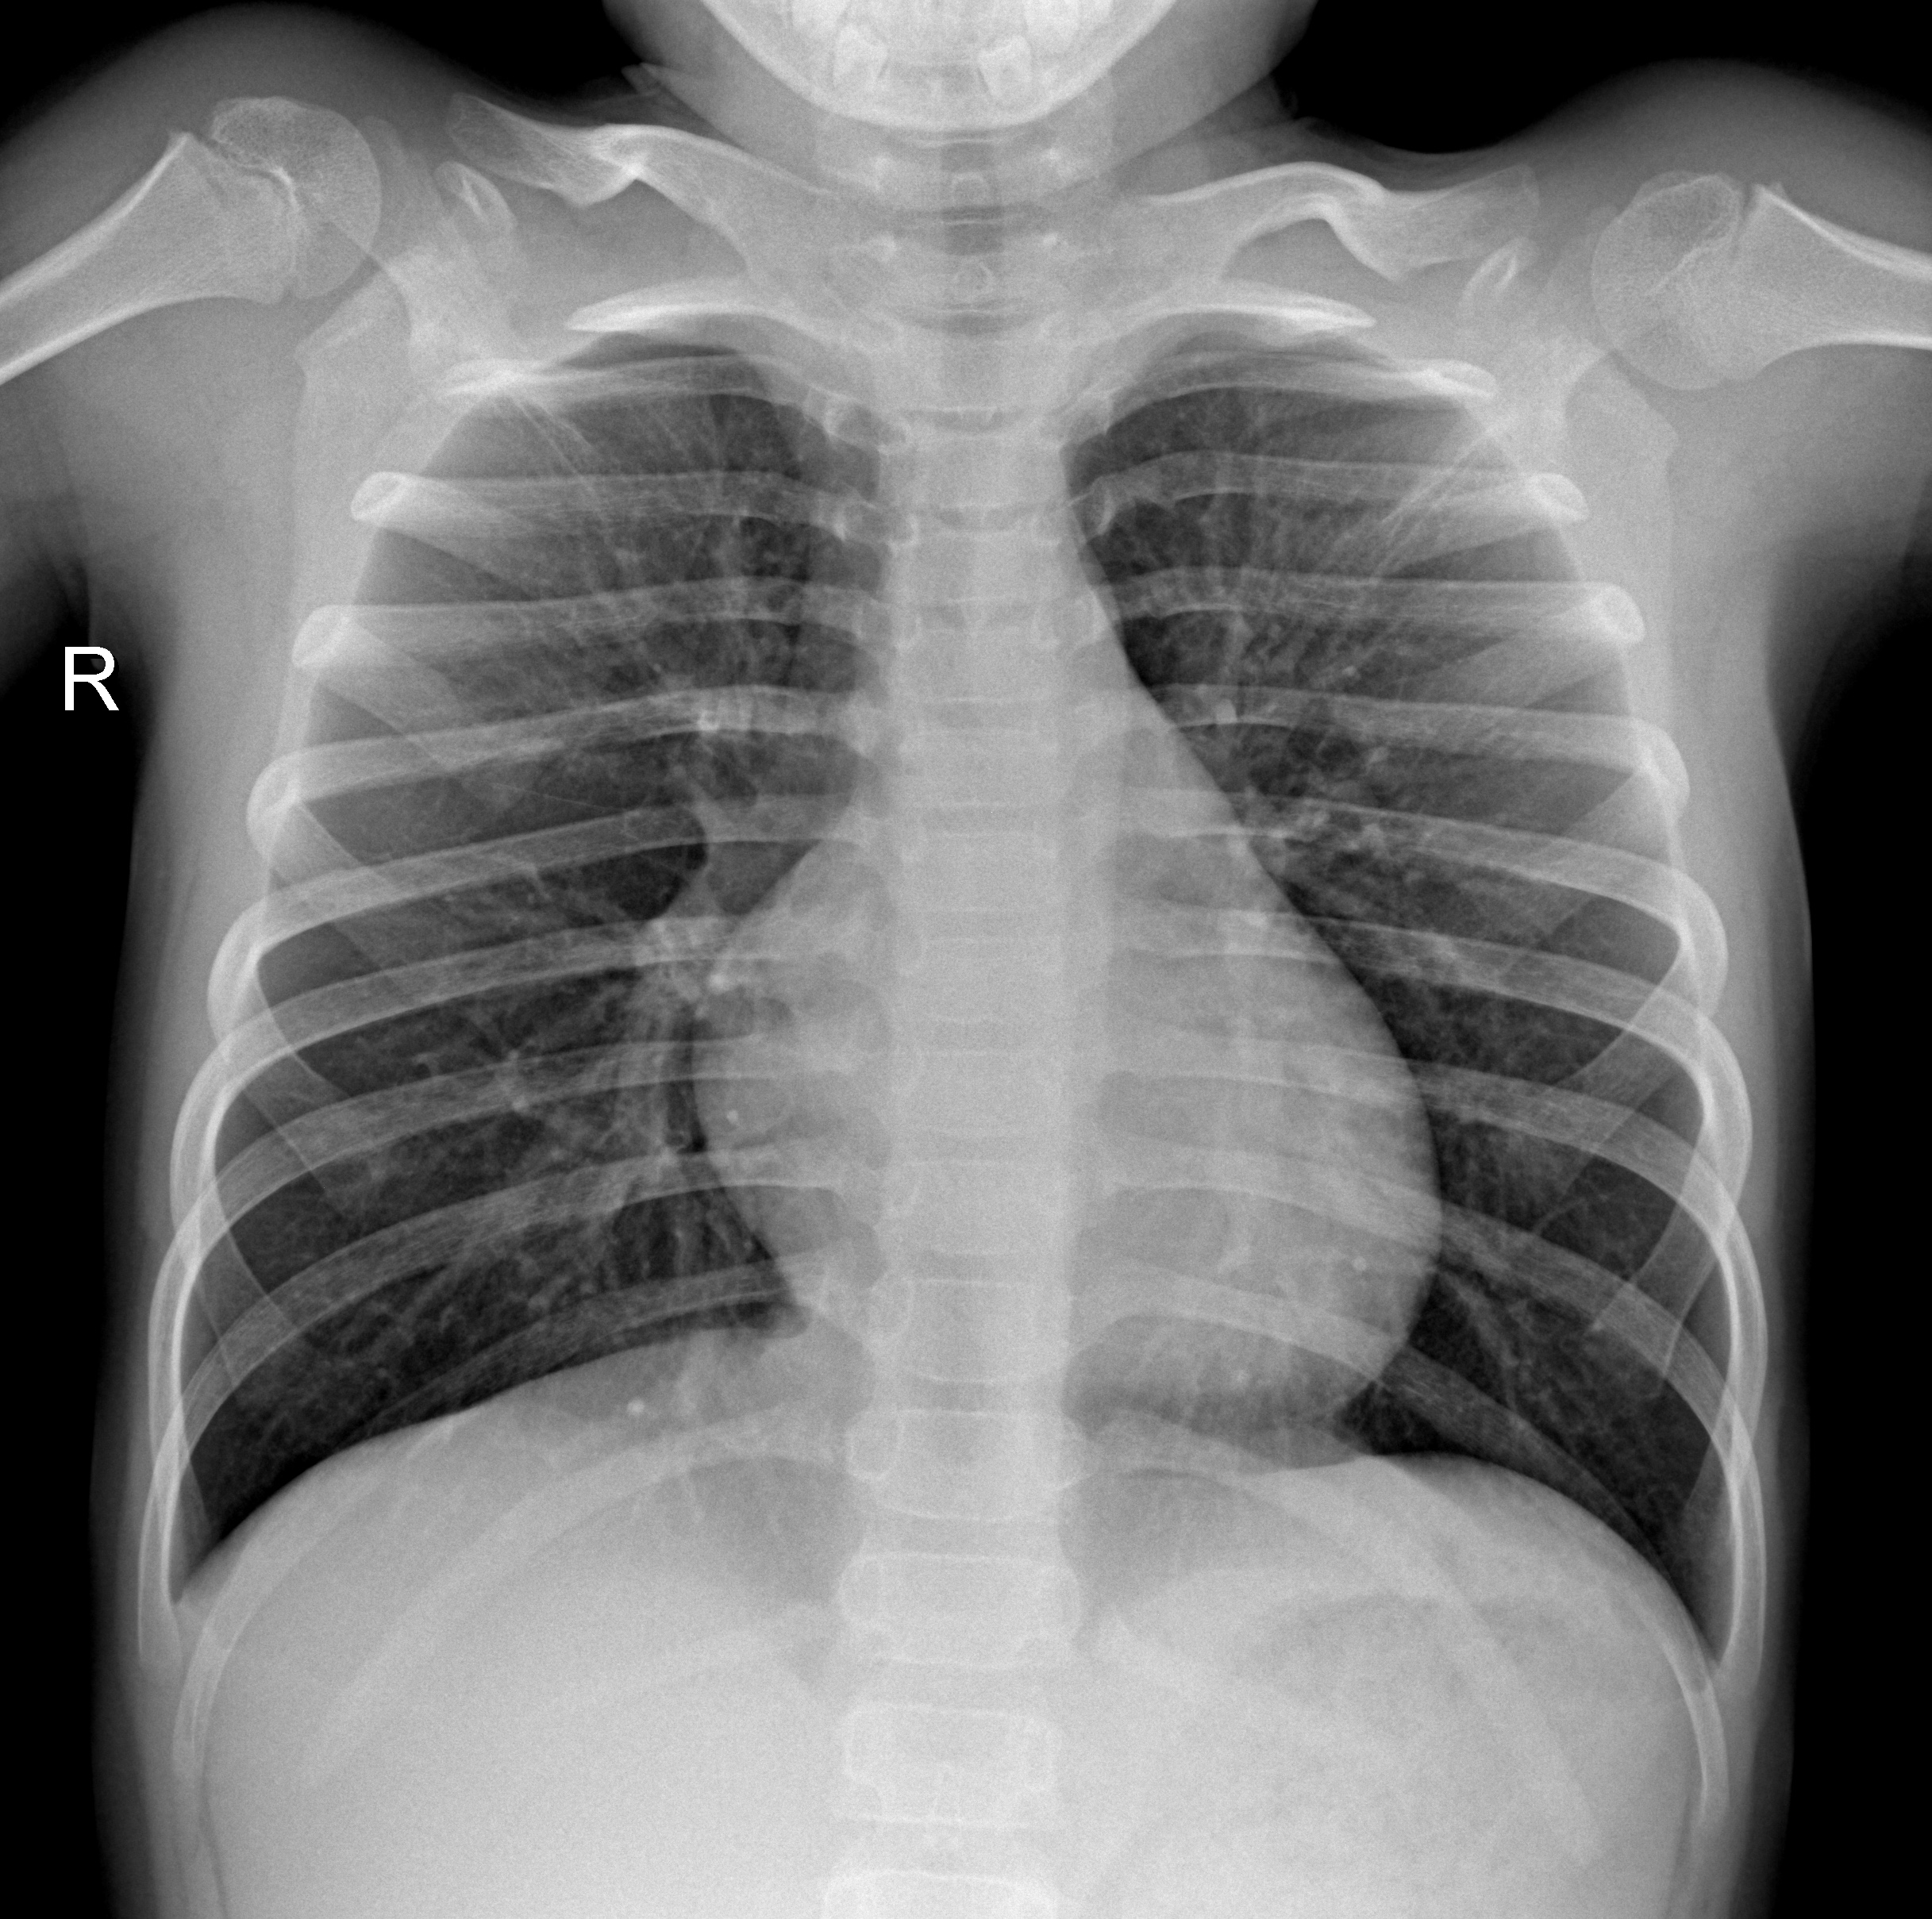
\includegraphics[width=0.4\textwidth]{Proposal/SampleNORMAL.jpeg}
    \caption{A sample image without pneumonia.\label{fig:SampleNORMAL}}
\end{figure}

\begin{figure}[H]
    \centering
    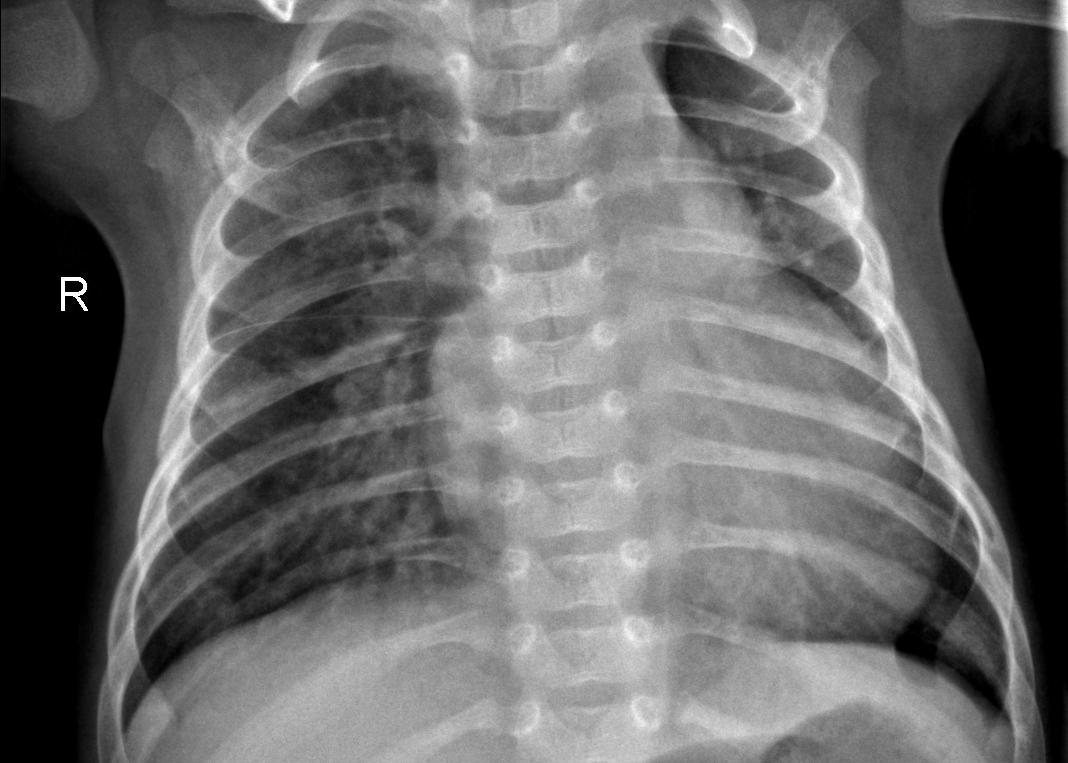
\includegraphics[width=0.5\textwidth]{Proposal/SamplePNEUMONIA.jpeg}
    \caption{A sample image with pneumonia.\label{fig:SamplePNEUMONIA}}
\end{figure}

\subsection{Potential issues}\label{sec:DatasetIssues}
The dataset has already been pre-emptively split into training and testing sets, which saves having to perform a manual split. 
However, the data itself is not immediately usable and will require further preprocessing before being used to train a model, namely due to the 
following issues:

\begin{itemize}
    \item Images are different resolutions.
    \begin{itemize}
        \item The sample images vary widely in resolution, with some being substantially higher than others.
        The neural network's input layer will be fixed in size, meaning all input data must be the 
        same size or the network will be unable to process it. This can be addressed programmatically using Keras to automatically resize 
        all images to a given resolution.
    \end{itemize}
    \item Class imbalance
    \begin{itemize}
        \item The training set contains 1,349 samples of patients without pneumonia, but 3,883 samples of patients with pneumonia.
        This will lead to the model favouring those with pneumonia rather than the underrepresented class of those without. This can be addressed 
        using the techniques discussed in Section \ref{sec:Augmentation}.
    \end{itemize}
\end{itemize}


% \begin{longtable}{ | p{0.25\textwidth} | p{0.65\textwidth} | }
%     \hline
%     \cellcolor{blue!25} Issue & \cellcolor{blue!25} Explanation \\
%     \hline
%     Images are not all the same resolution. & The neural network's input layer will be fixed in size, meaning all input data must be the 
%     same size or the network will be unable to process it. This can be addressed using Keras to automatically resize all images to a given 
%     resolution.\\
%     \hline
%     Class imbalance & The training set contains 1,349 samples of patients without pneumonia, but 3,883 samples of patients with pneumonia.
%     This will lead to the model favouring those with pneumonia rather than the underrepresented class of those without. This can be addressed 
%     using the techniques discussed in Section \ref{sec:Augmentation}.\\
%     \hline
%     \caption{The issues with the dataset before any preprocessing.}\label{tab:DatasetIssues}
% \end{longtable}

% ? 234 TestNorm, 390 TestPneu. 1349 TrainNorm, 3883 TrainPneu.

\pagebreak 

\section{Data science problem}
This dataset poses a clear data science problem pertaining to the binary classification of these images which will be addressed through the 
development of a convolutional neural network image classification model leveraging supervised learning. 
The ground truth is present within the dataset through its file structure\footnote{Because \textcite
{kermanyIdentifyingMedicalDiagnoses2018}'s work was not only on pneumonia, the Mendeley ZIP file contains two 
separate datasets. This proposal is only for the "chest\_xray" dataset.}, shown below:


\begin{verbatim}
    .
    `-- chest_xray/
        |-- test/
        |   |-- NORMAL/
        |   |   |-- NORMAL-4512-0001.jpeg
        |   |   |-- NORMAL-11419-0001.jpeg
        |   |   `-- ...234 more images
        |   `-- PNEUMONIA/
        |       |-- BACTERIA-40699-0001.jpeg
        |       |-- VIRUS-4190128-0001
        |       `-- ...388 more images
        `-- train/
            |-- NORMAL/
            |   |-- NORMAL-28501-0001.jpeg
            |   |-- NORMAL-32326-0001.jpeg
            |   `-- ...1347 more images
            `-- PNEUMONIA/
                |-- BACTERIA-7422-0001.jpeg
                |-- VIRUS-12220-0001.jpeg
                `-- ...3881 more images
\end{verbatim}

\noindent Files of the appropriate class are stored in the relevant subfolder\footnote{Shown file names are given as examples, and are not in the direct order they appear in the folders.}.
When this dataset is loaded, it will be possible to 
assign the relevant label to each image based on its subfolder of origin. Note that while there are separate files for bacterial and 
viral pneumonia, an analysis of other works using this dataset, seen in Chapter 2, indicated that this will not be an issue.

% "The aim is to develop a deep learning model to classify images into X classes."
% ? Describe the need for critical evaluation of the model.

% ! Footnote that the dataset contains multiple data science problems. I am only using "chest_xray", the 
% ! pneumonia identification problem.


\chapter{Related work}

% ! Added a ton of papers using this dataset to Zotero.
% ? You can use Litmaps to find more.

\section{Introduction}
This section of the report aims to demonstrate the main concepts
of related techniques that have been previously used to solve the problem 
through a thorough review of surrounding literature.

% ? What have other people done to solve it? How did they do it? 

\section{Traditional machine learning methods}
% ! This section was written while stressed-out and sleep-deprived and is likely absolute waffle that should be deleted.
Traditional machine learning methods such as Random Forests, K-Nearest Neighbours and Support 
Vector Machines have previously been leveraged for pneumonia classification as seen in the works of 
\textcite{ortiz-toroAutomaticDetectionPneumonia2022}. They state that leveraging these traditional approaches
alongside the creation of handcrafted textural features 'offers good performance with very low computational complexity',
as seen in their results wherein they attained an F1-Score
% ! Equation here for F1.
of 93\%.

\para However, leveraging traditional methods on detailed image datasets such as \textcite{kermanyIdentifyingMedicalDiagnoses2018}'s
relies upon manual feature engineering of textural features, which can unintentionally introduce bias. Dataset bias can significantly harm the generalisation capabilities of produced models \autocite{selvarajuGradCAMVisualExplanations2017}.
This is because it is possible that the new data given to a deployed model would differ from the preset features used on the original dataset,
which a biased model would be unable to accurately predict, unlike deep learning methods which can automatically interpret features without 
manual intervention.

\para Furthermore, some researchers such as \textcite{wangComparativeAnalysisImage2021} have leveraged both traditional and deep learning 
techniques on other unrelated datasets, wherein they discovered that the Support Vector Machine they used had an accuracy 10\% lower than 
a convolutional neural network on a large dataset, though actually had an accuracy 3\% higher on a smaller dataset. They also note that
deep learning methods have considerably longer training times than traditional counterparts.

\para SVMs in particular are the most commonly seen model in works using this dataset. SVMs aim to find the optimal hyperplane 
which separates one class from another. They are likely the most common due to their high performance and evaluation
metrics even when many dimensions are introduced, such as in image data. 

\begin{figure}[H]
    \centering
    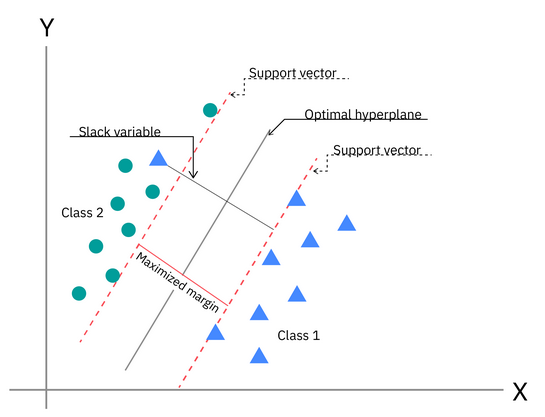
\includegraphics[width=0.5\textwidth]{Proposal/SVM.png}
    \caption{A cursory overview of an SVM's functionality \autocite{ibmWhatSupportVector2023}.\label{fig:SVM}}
\end{figure}


\section{Deep Neural Networks}
% * Neural networks themselves (Types [CNN, etc.])
Deep neural networks are the most heavily used methods for classification tasks with this dataset, which can be seen on both the 
dataset's Kaggle page \autocite{mooneyChestXRayImages2018}, and through a thorough literature search.

\para There are a wide variety of neural network 
types, though the most suitable and most commonly used neural network architecture across related literature\footnote{Specifically, the works of \textcite{elasnaouiDesignEnsembleDeep2021a,rajpurkarCheXNetRadiologistLevelPneumonia2017,sourabComparisonHybridDeep2022,stephenEfficientDeepLearning2019,umaribrahimConvolutionalNeuralNetwork2022b}} 
for image classifications such as the one proposed here is a Convolutional Neural Network (CNN).
CNNs are heavily used for image classification tasks across many fields, including for identifying pneumonia. A more detailed 
description of the functionality of a CNN can be found in Section \ref{sec:ModelArchitecture}, as this section instead details 
the accomplishments of other works with \textcite{kermanyIdentifyingMedicalDiagnoses2018}'s dataset.

\para \textcite{elasnaouiDesignEnsembleDeep2021a}'s work is one of the most informative\footnote{It should be noted that they used an altered dataset which they created from merging \textcite{kermanyIdentifyingMedicalDiagnoses2018}'s data with a COVID-19 dataset.},
%, and had their models also identify whether the pneumonia was from COVID or other causes.}, 
and tests three different pretrained CNNs and combinations of them merged into different ensemble models. 
They tested implementations of pretrained InceptionResNet\_V2, MobileNet\_V2, and ResNet50 models, achieving F1-scores of 93.52, 91.62 and 93.47 
respectively. They also produced an ensemble model containing all three, which achieved their highest F1 score of 94.84. Their work clearly 
depicts the effectiveness of CNNs in classifying pneumonia.

\para Analysing the works of others published on the dataset's Kaggle page also follows this trend - CNNs are the most optimal choice for this 
particular classification task, with many achieving accuracies of at least 92\% with minimal overfitting. 

\newpage

\section{Data augmentation and overfitting}\label{sec:Augmentation}
Many works on this dataset and related ones cite the previously mentioned class imbalance.
\textcite{mathurPneumoniaDetectionUsing2020} and others solve this using data augmentation, specifically to boost the number of samples without 
pneumonia so that the classes are balanced, thereby reducing bias in the eventual trained model.
To do so, they leverage the ImageDataGenerator from Keras to create artificial additional samples based on the original data through 
30-degree rotation, 20\% zoom, 10\% horizontal and/or vertical shifting, and horizontal flipping. These processes are all performed randomly,
and not always in the same order. This ensures a wide variety of differing samples for the model to train on, thereby greatly assisting 
the training process and eventual model performance metrics, as \textcite{mathurPneumoniaDetectionUsing2020} found with their model attaining 
an accuracy of 92.6\% and loss of 0.29 on the testing set after 11 epochs of training.

\begin{figure}[H]
    \centering
    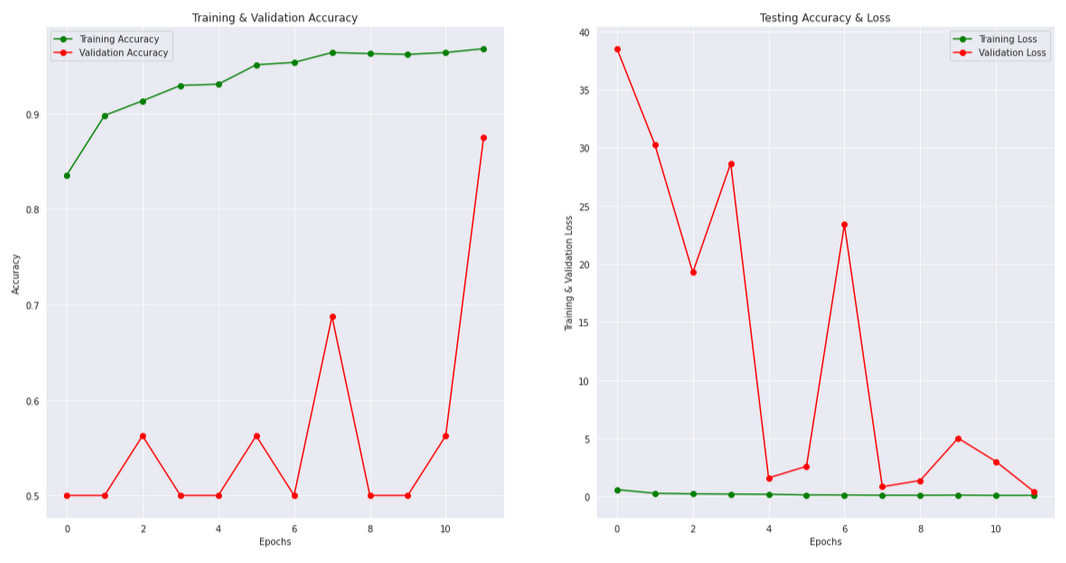
\includegraphics[width=0.8\textwidth]{Proposal/MathurModelMetrics.png}
    \caption{\textcite{mathurPneumoniaDetectionUsing2020}'s model performance over 11 epochs.\label{fig:MathurModelMetrics}}
\end{figure}

\noindent Through the graphs they generated, there were visible substantial improvements on the 11th epoch specifically, wherein validation 
accuracy and loss massively improved. This was likely found to be the perfect balance before the model started to overfit, which is defined 
as 'when an algorithm fits too closely or even exactly to its training data' \autocite{ibmWhatOverfittingIBM2021}. An overfit model would 
show patterns of excellent training accuracy and loss, but poor validation accuracy and loss, which could be seen notably on epochs 3 and 6
of \textcite{mathurPneumoniaDetectionUsing2020}'s work. If an overfit model was not remedied, it would perform terribly on real-world unseen 
data, which would go against the objectives of this project.  


\chapter{Deep learning fundamentals}

% ? CNNs are good for image classification because they identify 'features' of an image rather than just the entire image.
% ? For instance, if I train my network to recognise images of the number 5, what if the 5 was in the corner of the image and not the middle?
% ? A CNN wouldn't struggle with this, and would likely still identify it where other networks may not.

% ? Apparently, CNNs overfitting on smaller datasets is a big issue, hence why he wanted you to find one of decent size (which you did).
% ? Dropout is one technique to address this, but another interesting one is data augmentation such as image rotation.

% ? He likely wants you to do augmentation. Consider the computational risk of doing that, though, given you have 6000 images.
% * It might not be too bad, actually. CIFAR10 is slow because it's 60k images.

\section{What are deep neural networks?}
Deep neural networks are a significant advancement in computing which build greatly upon traditional 
machine learning techniques, especially in fields such as computer vision and image recognition. By leveraging newfound processing power 
typically found in modern graphics cards, \textbf{neural networks} formed of layers of neurons which replicate the functionality of 
the human mind can be created to solve problems at higher degrees of accuracy than ever before. A visualisation of a deep neural network 
is depicted in Figure \ref{fig:NeuralNetwork}, with key concepts detailed in Table \ref{tab:NeuralNetworkComponents}.

\begin{figure}[H]
    \centering
    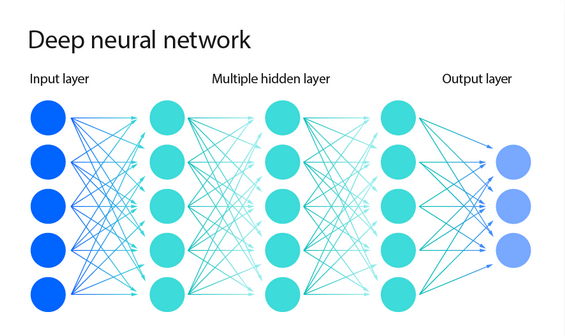
\includegraphics[width=0.8\textwidth]{Proposal/NeuralNetworkCropped.png}
    \caption{A neural network with input, hidden and output layers \autocite{ibmWhatNeuralNetwork2021}.\label{fig:NeuralNetwork}}
\end{figure}

\begin{longtable}{ | p{0.225\textwidth} | p{0.725\textwidth} | }
    \hline
    \cellcolor{blue!25} Concept & \cellcolor{blue!25} Description \\
    \hline
    Neuron & Similar to the human mind, neural networks are formed of synthetic neurons which receive, process and output one 
    data feature. All layers of a neural network are formed of neurons. \\
    \hline 
    Input layer & The first layer of any neural network, in which data is first taken into the network. Input layers 
    will be of a size equal to the amount of features; for example, a 32x32 image will need an input layer of 1024 neurons. \\
    \hline
    Hidden layers & The main processing logic of the neural network is performed in hidden layers. There can theoretically be any 
    amount of hidden layers in a network, though processing power requirements will grow exponentially. Hidden layers are executed sequentially,
    meaning that the first hidden layer will feed processed data directly into the second, and so on. This means that models with many hidden 
    layers ('deep models') will often yield higher accuracies, especially on their training data as they could begin to overfit. 
    Hidden layers can apply \textbf{weights} and \textbf{biases} to each neuron, which controls the importance of individual features 
    to the overall model.  \\
    \hline 
    Output layer & The final layer of any neural network, where a prediction is received. The output layer will contain neurons equal 
    to the number of classes in a classification problem (2 in binary, or $n$ in multi classification where $n$ is the number of classes),
    or exactly one neuron in a regression problem. In a classification problem,
    the neuron with the highest output is the predicted class. In a regression problem, the single output neuron directly outputs its
    prediction. \\
    \hline 
    Loss functions & Used to measure how well the model is predicting in relation to the actual target values in supervised learning.
    The loss function used is dependent on what problem the model is solving; regression tasks often use functions such as Mean Squared 
    Error (MSE), whereas classification tasks will use a cross-entropy function. The specific cross-entropy function once again depends 
    on the problem, with binary classification models often using Binary Cross-Entropy, whereas multi-class models will typically use 
    Categorical Cross-Entropy. The overall objective of a model is to minimise the value returned by these functions (the 'loss value').  \\
    \hline 
    Optimisers & Another key element in any neural network is the \textbf{optimiser}. There are a wide variety of options,
    with some of the most common being Stochastic Gradient Descent (SGD), RMSProp, or Adam. The objective of an optimiser 
    is to minimise model loss by dynamically adjusting the weights and learning rates of the network through a process called 
    \textbf{backpropagation}, which efficiently computes the gradient of the loss function while accounting for the 
    network's weights. \\
    \hline 
    Activation functions & Used to make a model 
    less linear, thereby allowing it to learn complex patterns in data, which is especially important when processing image data.
    The overall purpose of these functions are to dictate whether a neuron should activate (pass data on to the next layer) or not.
    If the neuron is activated, the output it receives is transformed based on its weights. Activation functions are essential 
    for backpropagation to ensure the model improves with each training epoch. Common activation functions include Rectified Linear 
    Unit (ReLU), Sigmoid and Softmax. Sigmoid and Softmax are particularly important in classification problems, with Sigmoid 
    outputting 0 or 1 for binary classification, and Softmax outputting probabilities for multi-class tasks. Because of this, an activation 
    function is often used on the output layer.   \\
    \hline 
    Epochs & The amount of times the model is trained on the data, affecting backpropagation as 
    weights and biases are calculated with each epoch. Too many epochs will eventually lead to 
    overfitting as the model becomes too calibrated to its training data and becomes unable 
    to generalise. \\
    \hline 
    Batch size & Not all data is given to the model at once during training for multiple reasons,
    one of the most important being memory usage. Large datasets use considerable amounts of memory,
    and RAM is a limited resource to the point where some datasets simply cannot fit in memory all 
    at once. Additionally, by using smaller batches, training can be faster and less computationally 
    intensive. \\
    \hline 
    Validation split & Data is typically split across three sets when training machine learning models.
    These sets are the training set encompassing the vast majority of the data that the model will 
    learn from, the testing set containing a small amount of data to evaluate the model's performance 
    on data it has never previously seen and is used after training has completed, 
    and the validation set containing a similar proportion of data 
    to the testing set which is used during training to evaluate performance on unseen data, which helps 
    to identify overfitting and to fine-tune hyperparameters.\\
    \hline 
    Hyperparameters & Epochs, batch size and validation split are a few examples of hyperparameters,
    which are used to determine the model's behaviour during training. It is an essential part of 
    model development to tune these hyperparameters to ensure the best possible model is produced. \\
    \hline
    \caption{Common concepts in any neural network.}\label{tab:NeuralNetworkComponents}
\end{longtable}


\section{Convolutional Neural Networks (CNNs)}
Convolutional Neural Networks (CNNs) are deep learning architectures designed to process data with a grid-like topology, such as images.
They consist of multiple specialised layers that extract hierarchical features from input data, enabling tasks like image classification and 
object detection. Table \ref{tab:CNNFeatures} details the key elements of CNNs.

\begin{longtable}{ | p{0.225\textwidth} | p{0.725\textwidth} | }
    \hline
    \cellcolor{blue!25} Feature & \cellcolor{blue!25} Description \\
    \hline
    Convolutional filter & Also sometimes referred to as a kernel. These filters are small matrices which effectively slide across 
    an image, creating a 'feature map', or convoluted feature. The filter \textbf{must} be smaller than the image itself. 
    A key feature of convolutional filters is that they use shared weights, ensuring that an object recognised in one part of an image 
    (the number 5 in the middle of the image, for example) can be recognised in a different part of an image. Early convolutional filters 
    will identify lower-level features such as large shapes, whereas further filters can learn deeper features such as specific objects 
    or human faces. \\
    \hline 
    Pooling layer & The feature map from convolutional filters cannot be directly passed into a new dense layer, and must first be 
    pooled. Pooling layers reduce the dimensionality of convolutional filters, downsampling them while retaining their key information
    by summarising features within select regions dependent on the pooling kernel size, which works similarly to the convolutional filter 
    size. There are two common pooling strategies: max pooling and average pooling, which are visually represented in Figure \ref{fig:Pooling}. \\
    \hline 
    Max pooling & When summarising each region, the maximum value is taken. This emphasises more prominent features in the image,
    while rejecting less prominent features. \\
    \hline 
    Average pooling & Computes the average value in each region, which allows more data to be retained at the possible expense of 
    not emphasising key details. \\
    \hline
    Stride & The stride of the convolutional or pooling kernel determines how far the kernel moves every time it takes a sample. 
    For example, a kernel with stride (2, 2) will move 2 pixels across to the right until it reaches the edge of the image, at which 
    point it will move 2 pixels down. This also applies to the pooling layer, where it would move 2 columns across the feature map. \\
    \hline
    \caption{Key features of Convolutional Neural Networks.}\label{tab:CNNFeatures}
\end{longtable}

\begin{figure}[H]
    \centering
    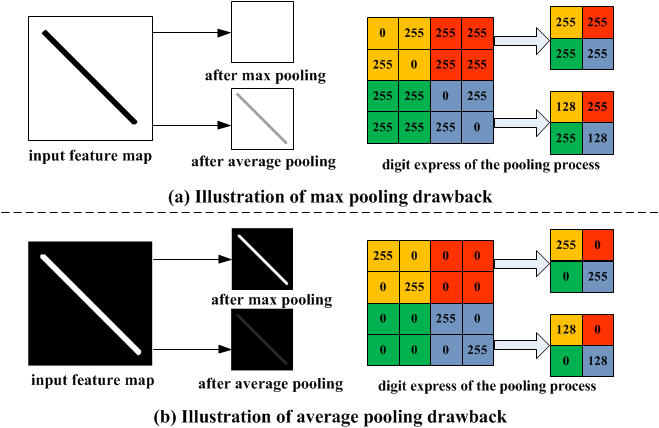
\includegraphics[width=\textwidth]{Proposal/PoolingLayers.png}
    \caption{An example of average and max pooling \autocite{yuMixedPoolingConvolutional2014}.\label{fig:Pooling}}
\end{figure}


\chapter{Proposed model}
\section{Architecture}\label{sec:ModelArchitecture}
As evidenced by the review of related work conducted across Chapter 2, the most suitable model for
classifying the pneumonia chest X-rays will be a CNN due to their high proficiency in identifying image 
features compared to other models. Unfortunately, training a CNN to a good degree of accuracy requires 
immense amounts of training data which will not be found in this dataset alone. As such, it will be 
best to leverage pretrained models such as ResNet50 or EfficientNet due to their large training 
corpus and high performance even in scenarios with class imbalance such as the one presented by this 
dataset. The model will then have additional layers added for this specific binary classification task.

\section{Preprocessing}
% ! Perhaps remove the earlier mention of the dataset's issues, instead moving it to here.
\para As mentioned previously in Section \ref{sec:DatasetIssues}, the dataset's images are not
all the same resolution, and a class imbalance is present, so significant preprocessing steps will need 
to be taken; most notably data augmentation and image resizing. In doing so, we can ensure that all 
data fed to the input layer is consistent and usable in training and evaluating\footnote{While data from the testing set will be resized so that it can be used as input for evaluation, it will not be augmented, as this would defeat the purpose of a train/test split.} 
the network.

% ? Write about multiple models.
\section{Evaluation strategy}
% ? How will you evaluate your results? Confusion matrix, F1?
The model's performance against its testing data will be thoroughly evaluated, primarily using accuracy, loss and F1-Score as key metrics.
Accuracy is defined as the total number of correct classifications (positive and negative) divided by the total number of samples,
which can be visualised as:

\begin{equation}\label{eq:Accuracy}
    \text{Accuracy} = \frac{\text{TP} + \text{TN}}{\text{TP} + \text{TN} + \text{FP} + \text{FN}}
\end{equation}

\para F1-Score is the harmonic mean of the model's precision and recall, providing an equally weighted combination of both statistics as one 
metric. It is particularly useful with imbalanced datasets, including medical datasets, where false classifications can have dire consequences.

\begin{equation}\label{eq:Recall}
    \text{Recall} = \frac{\text{TP}}{\text{TP} + \text{FN}}
\end{equation}

\begin{equation}\label{eq:Precision}
    \text{Precision} = \frac{\text{TP}}{\text{TP} + \text{FP}}
\end{equation}

\begin{equation}\label{eq:F1Score}
    \text{F1-Score} = 2 \times \frac{\text{Precision} \times \text{Recall}}{\text{Precision} + \text{Recall}}
\end{equation}

\newpage 

\para Additionally, visualising the performance of a classification model can be performed using a confusion matrix, which is a simple grid 
showing the amount of data that was correctly classified as positive ('true positive'), negative ('true negative'), and incorrectly classified
('false positive', 'false negative'). An example of a confusion matrix is depicted in Figure \ref{fig:ConfusionMatrix}.

\begin{figure}[H]
    \centering
    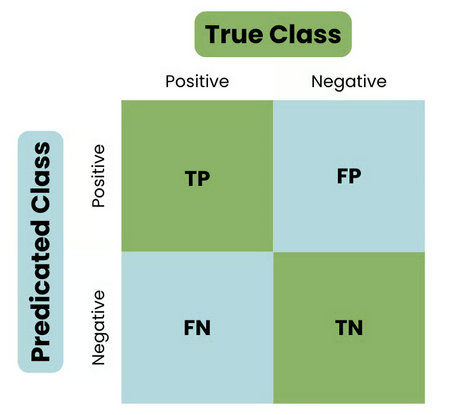
\includegraphics[width=0.5\textwidth]{Proposal/ConfusionMatrix.png}
    \caption{An example confusion matrix \autocite{datacampWhatConfusionMatrix}. \label{fig:ConfusionMatrix}}
\end{figure}


% ? The model proposed here doesn't *need* to be the one you eventually use, but you should.

% ! Add the word count to the title page before submission.
% ! Approximately 1800 currently? Not certain as tables are included by texcount.

% ? When you submit your code, don't use your coloured comments like these.

\addcontentsline{toc}{chapter}{Bibliography}

% ? Prevents bibliography overflowing hbox at the expense of it taking up more lines on the page.
\emergencystretch=1em
\printbibliography


\end{document}